% !TEX root = ../main.tex
% SECTION 11: ELEKTROMOTOREN
% Inhalt: Liv Erne, Silvio Seiz — Form: ZSF-Template-Rework
% ============================================================

\StartChapter[ch:elektromotoren]{Elektromotoren}
\ZSFindex{Elektromotor}

\SubsectionBar[sec:dc-motoren]{DC-Motoren (Permanentmagneterregte Gleichstrommotoren)}
\ZSFindex{DC-Motor}
\ZSFindexsee{Gleichstrommotor}{DC-Motor}

\ZSFfig[0.9]{graphics/v13_dc_motor_aufbau.png}{}{}

\begin{runintext}
\ZSFReadableOn
\ZSFkeyword{Stator}:~ortsfestes Magnetfeld. \ZSFkeyword{Rotor}:~Spulen erzeugen Drehbewegung durch Anziehung/Abstossung. \ZSFkeyword{Kommutator}:~mitdrehende Ringsegmente + ortsfeste Kohlebürsten wechseln Stromrichtung in Spulen bei Drehung.
\end{runintext}

\begin{figbox}[Vor und nach Stromrichtungswechsel]
\centering
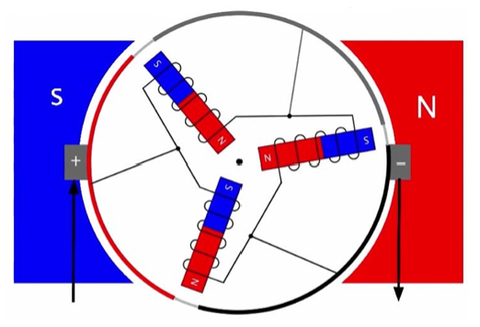
\includegraphics[width=0.27\linewidth,keepaspectratio]{graphics/v13_dc_motor_vor_stromrichtungswechsel.png}\quad
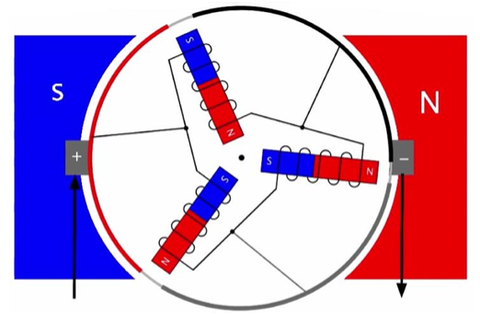
\includegraphics[width=0.27\linewidth,keepaspectratio]{graphics/v13_dc_motor_nach_stromrichtungswechsel.png}
\end{figbox}

\begin{formulabox}[Kennwerte \& Konstanten]
$1\cdot \dfrac{A}{mNm} = 60'000 \cdot \dfrac{min^{-1}}{V}$

$\ZSFmotorKn = \dfrac{1}{2\pi \ZSFmotorKm}\, [\dfrac{s^{-1}}{V}] \rightarrow \cdot 60 = [\dfrac{min^{-1}}{V}]$

$\ZSFmotorKm = \dfrac{\ZSFmotorM}{\ZSFmotorI} \qquad \ZSFmotorIZero = \dfrac{\ZSFmotorMR}{\ZSFmotorKm}$
\formulanote{$\ZSFmotorKn$:~Drehzahlkonst., $\ZSFmotorKm$:~Drehmomentkonst.}
\end{formulabox}

\phantomsection\label{formula:motor-drehzahl}
\begin{formulabox}[Drehzahl]
$\ZSFmotorN = \ZSFmotorKn \cdot \ZSFmotorU \ [min^{-1}] \qquad \ZSFmotorNZero = \ZSFmotorKn \cdot (\ZSFmotorUN - \ZSFmotorIZero \cdot \ZSFmotorR)$

$\ZSFmotorN = \ZSFmotorKn \cdot (\ZSFmotorUN - \ZSFmotorIZero \cdot \ZSFmotorR) - \dfrac{\ZSFmotorKn}{\ZSFmotorKm}\cdot \ZSFmotorR \cdot \ZSFmotorM = \ZSFmotorNZero - \dfrac{\ZSFmotorNZero \cdot \ZSFmotorM}{\ZSFmotorMH}$
\formulanote{$\ZSFmotorUN$:~Nennspannung \ $\cdot$ \ $\ZSFmotorIZero$:~Leerlaufstrom \ $\cdot$ \ $\ZSFmotorNZero$:~Leerlaufdrehzahl \ $\cdot$ \ $\ZSFmotorR$:~Wicklungswiderstand}
\end{formulabox}

\begin{splitbox}[0.39]
  \begin{figbox}[Motorkennlinien]
    \centering
    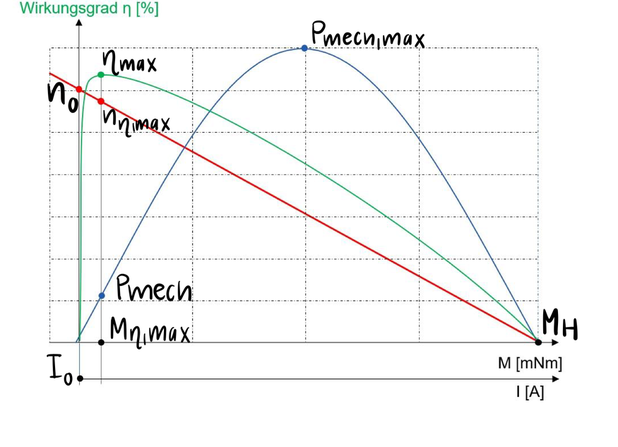
\includegraphics[width=\linewidth,keepaspectratio]{graphics/dc_motor_motorkennlinien_drehmoment_wirkungsgrad_leistung.png}
  \end{figbox}
\tcblower
  \phantomsection\label{formula:motor-drehmoment}
  \begin{formulabox}[Drehmoment]
    \centering
    $\displaystyle \ZSFmotorM = \ZSFmotorKm \cdot \ZSFmotorI \qquad \ZSFmotorMR = \ZSFmotorIZero\cdot \ZSFmotorKm$
    \par\vskip\ZSFspaceXS
    $\displaystyle \ZSFmotorMH = \dfrac{\ZSFmotorNZero \ZSFmotorKm}{\ZSFmotorKn \ZSFmotorR} = (\ZSFmotorUN - \ZSFmotorIZero \ZSFmotorR)\cdot \dfrac{\ZSFmotorKm}{\ZSFmotorR}$
    \par\vskip\ZSFspaceXS
    $\displaystyle \ZSFmotorMMechMax = \dfrac{\ZSFmotorMH - \ZSFmotorMR}{2}$
    \par\vskip\ZSFspaceXS
    $\displaystyle \ZSFmotorMEtaMax = \sqrt{\ZSFmotorMH \cdot \ZSFmotorMR}$
    \formulanote{$\ZSFmotorMH$:~Anhaltemoment, $\ZSFmotorMR$:~Reibmoment}
  \end{formulabox}
\end{splitbox}

\begin{formulabox}[Leistung \& Wirkungsgrad]
\formulasources{$\ZSFmotorN$:~\ZSFsource{aus}{formula:motor-drehzahl}, $\ZSFmotorM$:~\ZSFsource{aus}{formula:motor-drehmoment} \ $\cdot$ \ $\ZSFmotorNZero$:~nur Leerlauf}
$\ZSFmotorPEl = \ZSFmotorU \cdot \ZSFmotorI = \ZSFmotorR \cdot \ZSFmotorI^2 + \ZSFmotorM\cdot 2\pi \ZSFmotorN \qquad \ZSFmotorPMech = 2\pi \ZSFmotorN \ZSFmotorM$

$\ZSFmotorPMechMax = \dfrac{\ZSFmotorR}{4}\cdot (\dfrac{\ZSFmotorUN}{\ZSFmotorR} - \ZSFmotorIZero)^2$

$\ZSFmotorEta = \dfrac{\ZSFmotorPMech}{\ZSFmotorPEl} = \dfrac{-\ZSFmotorR\cdot \ZSFmotorI^2 + (\ZSFmotorU+\ZSFmotorR\cdot \ZSFmotorIZero)\cdot \ZSFmotorI - \ZSFmotorU\cdot \ZSFmotorIZero}{\ZSFmotorU\cdot \ZSFmotorI}$

$\ZSFmotorEtaMax = (1-\sqrt{\dfrac{\ZSFmotorIZero \cdot \ZSFmotorR}{\ZSFmotorUN}})^2$
\end{formulabox}


\ZSFindex{Motorkennlinie}
\ZSFindex{Drehzahlkonstante}
\ZSFindex{Drehmomentkonstante}
\ZSFindex{Anhaltemoment}

\SubsectionBar[sec:servos]{Servos (Geregelte Antriebssysteme)}
\ZSFindex{Servo}

\begin{splitbox}[0.46]
\centering
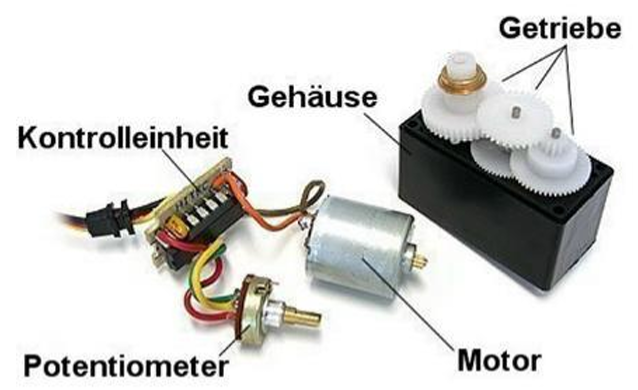
\includegraphics[width=\linewidth,keepaspectratio]{graphics/v13_servo_aufbau_motor_getriebe_potentiometer.png}
\tcblower
\ZSFReadableOn
Ist-Position wird gemessen und mit Soll-Position verglichen. Bei Differenz wird der Motor aktiviert, bis Soll erreicht. Der \ZSFkeyword{Potentiometer} ändert seinen Widerstand je nach Drehwinkel $\ZSFmotorPhi$. Drehbereich: $270^\circ$.
\end{splitbox}

\ZSFfig[0.9]{graphics/v13_servo_blockdiagramm_funktion.png}{}{}

\SubsectionBar[sec:stepper]{Stepper (Hybridschrittmotoren)}
\ZSFindex{Stepper}
\ZSFindexsee{Schrittmotor}{Stepper}

\begin{defbox}[Aufbau]
\ZSFReadableOn
Rotor aus axial magnetisierten \ZSFkeyword{Permanentmagneten} mit gezahnten Polscheiben. Stator aus Kupferspulen mit innenverzahnten Ringsegmenten. Gleiche Teilung, aber Segmente verschoben — nur zwei gegenüberliegende Segmente gleich ausgerichtet.

\formulasep
\noindent
\begin{minipage}[c]{0.48\linewidth}
\centering
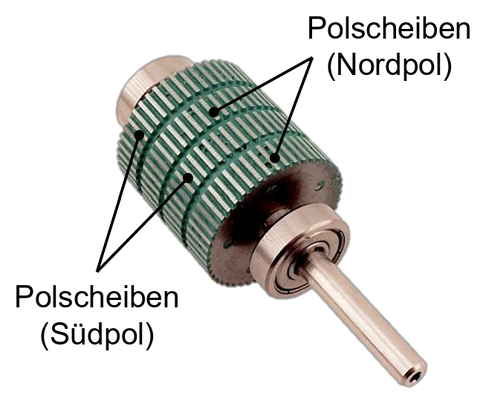
\includegraphics[width=0.75\linewidth,keepaspectratio]{graphics/v13_schrittmotor_aufbau_rotor_polscheiben.png}
\end{minipage}\hfill
\begin{minipage}[c]{0.48\linewidth}
\centering
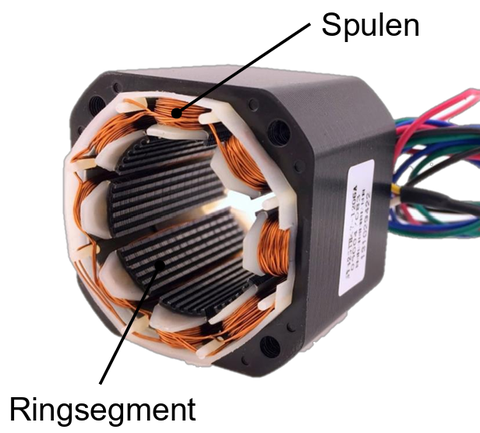
\includegraphics[width=0.75\linewidth,keepaspectratio]{graphics/v13_schrittmotor_aufbau_stator_spulen.png}
\end{minipage}
\end{defbox}

\begin{defbox}[Funktionsweise \& Betriebsarten]
\ZSFReadableOn
\ZSFkeyword*{Funktionsweise}:~Rotation durch schrittweises Spulen-Aktivieren. Gegenüberliegende Spulen zeitgleich \& gleichgerichtet. Versatz um $\tau/2$ $\rightarrow$ max. Anziehung/Abstossung.
\par\formulasep
\noindent
\begin{minipage}[c]{0.48\linewidth}
\centering
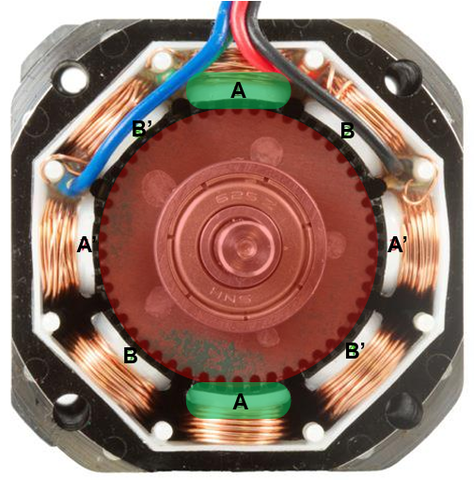
\includegraphics[width=0.72\linewidth,keepaspectratio]{graphics/v13_schrittmotor_unipolarer_betrieb.png}
\end{minipage}\hfill
\begin{minipage}[c]{0.48\linewidth}
\centering
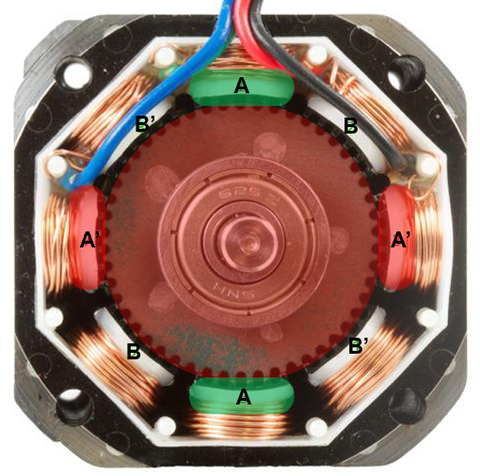
\includegraphics[width=0.72\linewidth,keepaspectratio]{graphics/v13_schrittmotor_bipolarer_betrieb.png}
\end{minipage}
\par\formulasep
\ZSFdanger{Uhrzeigersinn!} bei folgenden Aktivierungsfolgen:
\par\ZSFgapXS
\begin{ZSFtable}[\ZSFfontTableDense]{Z{1.4} Z{1.0} Z{0.9} Z{0.9} Z{0.9} Z{0.9}}
  \ZSFheaderRow
  \ZSFhead{Betrieb} & \ZSFhead{Schritt} & \ZSFhead{A} & \ZSFhead{B} & \ZSFhead{A'} & \ZSFhead{B'} \\
  Unipolar & Halb & grün & grün & aus & aus \\
  Unipolar & Voll & aus & grün & aus & aus \\
  Bipolar & Halb & grün & grün & rot & rot \\
  Bipolar & Voll & aus & grün & aus & rot
\end{ZSFtable}
\par\ZSFgapXS
\ZSFdanger{Halbschritt: Drehmomentschwankung (ungerade Spulenpaare).}\par\ZSFgapXS
\ZSFdanger{Bipolar: höheres Haltemoment, tiefer Wirkungsgrad.}
\end{defbox}
\ZSFindex{unipolarer Betrieb}
\ZSFindex{bipolarer Betrieb}
